\subsection{Termux}
\begin{enumerate}[label=\arabic*.,ref=\theenumi]
	\item On your android device, follow the instructions in 
%fdroid apk from
%
\begin{lstlisting}
https://github.com/gadepall/fwc-1
\end{lstlisting}
to setup and install Debian on Termux.
\iffalse
\item Install Termux from apkpure
\item Install basic packages on termux 
\begin{lstlisting}
#Give termux access to your  user directory in android
termux-setup-storage

#Upgrade packages
apt update && apt upgrade
apt install build-essential openssh

#Mandatory packages
apt install curl git wget subversion proot proot-distro python  nmap neovim ranger
#------------------End Install Termux----------------------------
\end{lstlisting}
\item Install debian on termux 
\begin{lstlisting}
proot-distro install debian
proot-distro login debian
\end{lstlisting}
\fi
\end{enumerate}
\subsection{Platformio }
\begin{enumerate}[label=\arabic*.,ref=\theenumi]
\item Follow the instructions in 
\begin{lstlisting}
https://docs.platformio.org/en/stable/core/installation/methods/installer-script.html#super-quick-macos-linux
\end{lstlisting}
to install platformio.
\item Execute the following on debian
\begin{lstlisting}
cd ide/piosetup/codes
pio run
\end{lstlisting}
% Insert your image here
\begin{center}
    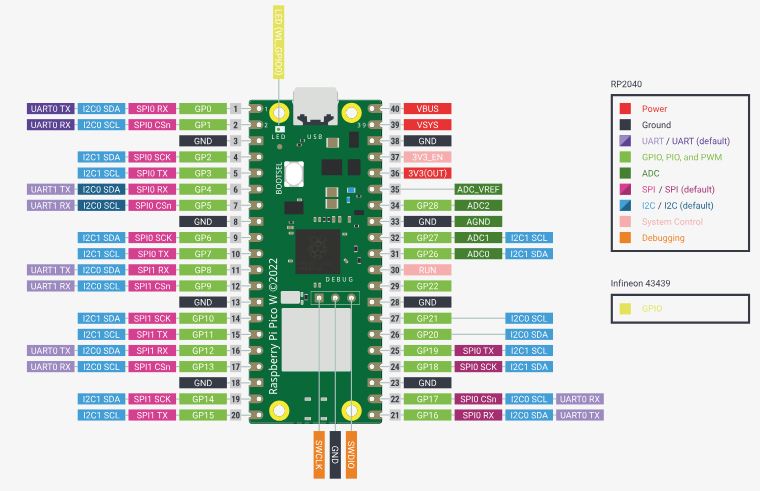
\includegraphics[width=0.6\textwidth, height=0.3\textheight]{installation/picowpinout.jpg}
    \vspace{0.5em} % Adjust the amount of space as needed
    \captionof{figure}{Pin Diagram} % Adds a centered caption under the image
\end{center}
\vspace{0.5em} % Adjust the amount of space as needed
\item Connect RUN on pico W to GND. Keep pressing BOOTSEL while removing the RUN-GND wire from GND.Pico W is now ready to be flashed.
\begin{lstlisting}
Downlaod EtchDroid from playstore.Flash the uf2 file using EtchDroid.
\end{lstlisting}
\vspace{0.5em} % Adjust the amount of space as needed
\item The Onboard LED will start blinking.
\end{enumerate}





